\documentclass[border=0.125cm]{standalone}

\usepackage{graphicx}
\usepackage{color}
\usepackage{tikz}
\usepackage{pgfplots}
\usepackage{pgf-umlsd}
\usepackage{ifthen}

\begin{document}

	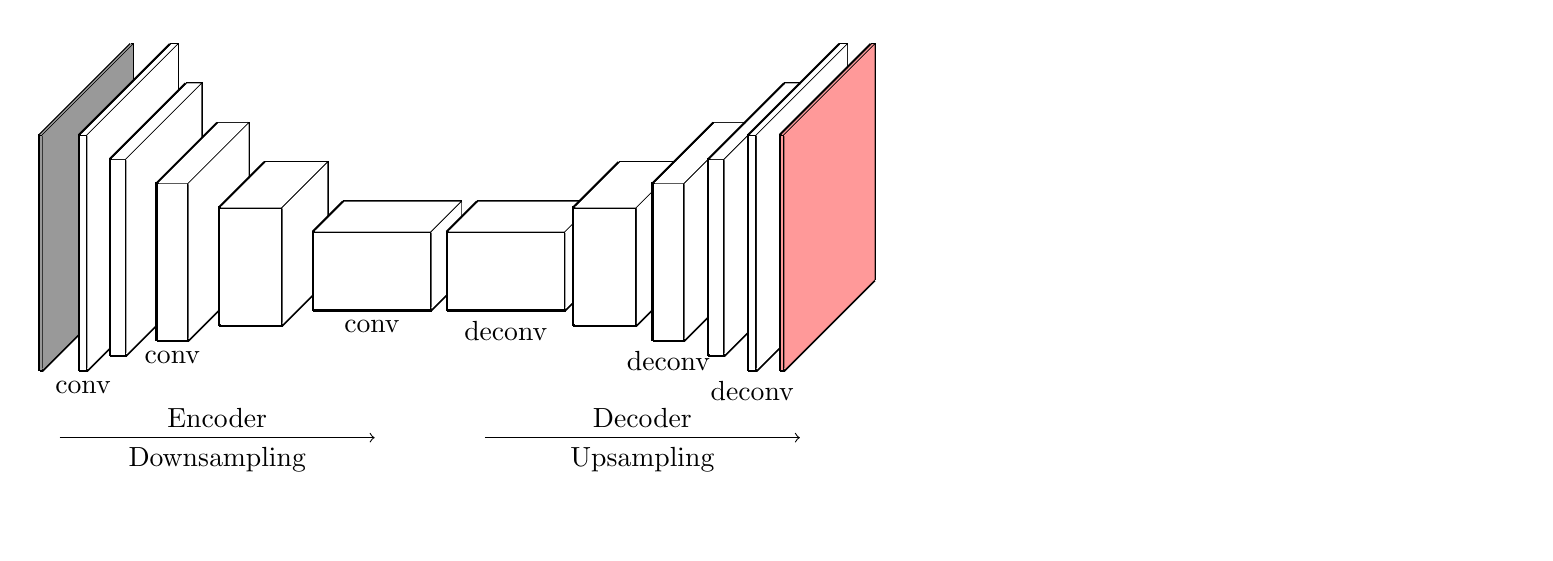
\begin{tikzpicture}
		\draw[use as bounding box, transparent] (-1.8,-3.2) rectangle (17.2, 3.2);

		% 1st argument: Height and width of the layer rectangle slice.
		% 2nd argument: Depth of the layer slice
		% 3rd argument: X Offset --> use it to offset layers from previously drawn layers.
		% 4th argument: Options for filldraw.
		% 5th argument: Text to be placed below this layer.
		% 6th argument: Y Offset --> Use it when an output needs to be fed to multiple layers that are on the same X offset.

		\newcommand{\networkLayer}[6]{
			\def\a{#1} % Input resolution for current layer.
			\def\b{0.02}
			\def\c{#2} % Width of the cube to distinguish number of input channels for current layer.
			\def\t{#3} % X offset for current layer.
			\def\d{#4} % Y offset for current layer.

			% Draw the layer body.
			\draw[line width=0.3mm](\c+\t,0,\d) -- (\c+\t,\a,\d) -- (\t,\a,\d);                                                      % back plane
			\draw[line width=0.3mm](\t,0,\a+\d) -- (\c+\t,0,\a+\d) node[midway,below] {#6} -- (\c+\t,\a,\a+\d) -- (\t,\a,\a+\d) -- (\t,0,\a+\d); % front plane
			\draw[line width=0.3mm](\c+\t,0,\d) -- (\c+\t,0,\a+\d);
			\draw[line width=0.3mm](\c+\t,\a,\d) -- (\c+\t,\a,\a+\d);
			\draw[line width=0.3mm](\t,\a,\d) -- (\t,\a,\a+\d);

			% Recolor visible surfaces
			\filldraw[#5] (\t+\b,\b,\a+\d) -- (\c+\t-\b,\b,\a+\d) -- (\c+\t-\b,\a-\b,\a+\d) -- (\t+\b,\a-\b,\a+\d) -- (\t+\b,\b,\a+\d); % front plane
			\filldraw[#5] (\t+\b,\a,\a-\b+\d) -- (\c+\t-\b,\a,\a-\b+\d) -- (\c+\t-\b,\a,\b+\d) -- (\t+\b,\a,\b+\d);

			% Colored slice.
			\ifthenelse {\equal{#5} {}}
			{} % Do not draw colored slice if #4 is blank.
			{\filldraw[#5] (\c+\t,\b,\a-\b+\d) -- (\c+\t,\b,\b+\d) -- (\c+\t,\a-\b,\b+\d) -- (\c+\t,\a-\b,\a-\b+\d);} % Else, draw a colored slice.
		}

		% INPUT
		\networkLayer{3.0}{0.03}{-0.5}{0.0}{color=gray!80}{}

		% ENCODER
		\networkLayer{3.0}{0.1}{0.0}{0.0}{color=white}{conv}   % E1
		\networkLayer{2.5}{0.2}{0.2}{0.0}{color=white}{}    	% E2
		\networkLayer{2.0}{0.4}{0.6}{0.0}{color=white}{conv}    % E3
		\networkLayer{1.5}{0.8}{1.2}{0.0}{color=white}{}    	% E4
		\networkLayer{1.0}{1.5}{2.2}{0.0}{color=white}{conv}    % E5
		
		\draw[->] (-1.4,-2)--node[below,align=center]{Downsampling}node[above,align=center]{Encoder}(2.6,-2) ;
		% DECODER
		\networkLayer{1.0}{1.5}{3.9} {0.0}{color=white}{deconv} 	% D1
		\networkLayer{1.5}{0.8}{5.7}{0.0}{color=white}{} 			% D2
		\networkLayer{2.0}{0.4}{6.9}{0.0}{color=white}{deconv}      % D3
		\networkLayer{2.5}{0.2}{7.8}{0.0}{color=white}{}       		% D4
		\networkLayer{3.0}{0.1}{8.5}{0.0}{color=white}{deconv}      % D5
		\draw[->] (4,-2)--node[below,align=center]{Upsampling}node[above,align=center]{Decoder}(8,-2) ;
		% OUTPUT
		\networkLayer{3.0}{0.05}{8.9}{0.0}{color=red!40}{}          % Reconstructed image


	\end{tikzpicture}

\end{document}